\documentclass[twoside]{book}

% Packages required by doxygen
\usepackage{fixltx2e}
\usepackage{calc}
\usepackage{doxygen}
\usepackage[export]{adjustbox} % also loads graphicx
\usepackage{graphicx}
\usepackage[utf8]{inputenc}
\usepackage{makeidx}
\usepackage{multicol}
\usepackage{multirow}
\PassOptionsToPackage{warn}{textcomp}
\usepackage{textcomp}
\usepackage[nointegrals]{wasysym}
\usepackage[table]{xcolor}

% Font selection
\usepackage[T1]{fontenc}
\usepackage[scaled=.90]{helvet}
\usepackage{courier}
\usepackage{amssymb}
\usepackage{sectsty}
\renewcommand{\familydefault}{\sfdefault}
\allsectionsfont{%
  \fontseries{bc}\selectfont%
  \color{darkgray}%
}
\renewcommand{\DoxyLabelFont}{%
  \fontseries{bc}\selectfont%
  \color{darkgray}%
}
\newcommand{\+}{\discretionary{\mbox{\scriptsize$\hookleftarrow$}}{}{}}

% Page & text layout
\usepackage{geometry}
\geometry{%
  a4paper,%
  top=2.5cm,%
  bottom=2.5cm,%
  left=2.5cm,%
  right=2.5cm%
}
\tolerance=750
\hfuzz=15pt
\hbadness=750
\setlength{\emergencystretch}{15pt}
\setlength{\parindent}{0cm}
\setlength{\parskip}{3ex plus 2ex minus 2ex}
\makeatletter
\renewcommand{\paragraph}{%
  \@startsection{paragraph}{4}{0ex}{-1.0ex}{1.0ex}{%
    \normalfont\normalsize\bfseries\SS@parafont%
  }%
}
\renewcommand{\subparagraph}{%
  \@startsection{subparagraph}{5}{0ex}{-1.0ex}{1.0ex}{%
    \normalfont\normalsize\bfseries\SS@subparafont%
  }%
}
\makeatother

% Headers & footers
\usepackage{fancyhdr}
\pagestyle{fancyplain}
\fancyhead[LE]{\fancyplain{}{\bfseries\thepage}}
\fancyhead[CE]{\fancyplain{}{}}
\fancyhead[RE]{\fancyplain{}{\bfseries\leftmark}}
\fancyhead[LO]{\fancyplain{}{\bfseries\rightmark}}
\fancyhead[CO]{\fancyplain{}{}}
\fancyhead[RO]{\fancyplain{}{\bfseries\thepage}}
\fancyfoot[LE]{\fancyplain{}{}}
\fancyfoot[CE]{\fancyplain{}{}}
\fancyfoot[RE]{\fancyplain{}{\bfseries\scriptsize Generated by Doxygen }}
\fancyfoot[LO]{\fancyplain{}{\bfseries\scriptsize Generated by Doxygen }}
\fancyfoot[CO]{\fancyplain{}{}}
\fancyfoot[RO]{\fancyplain{}{}}
\renewcommand{\footrulewidth}{0.4pt}
\renewcommand{\chaptermark}[1]{%
  \markboth{#1}{}%
}
\renewcommand{\sectionmark}[1]{%
  \markright{\thesection\ #1}%
}

% Indices & bibliography
\usepackage{natbib}
\usepackage[titles]{tocloft}
\setcounter{tocdepth}{3}
\setcounter{secnumdepth}{5}
\makeindex

% Hyperlinks (required, but should be loaded last)
\usepackage{ifpdf}
\ifpdf
  \usepackage[pdftex,pagebackref=true]{hyperref}
\else
  \usepackage[ps2pdf,pagebackref=true]{hyperref}
\fi
\hypersetup{%
  colorlinks=true,%
  linkcolor=blue,%
  citecolor=blue,%
  unicode%
}

% Custom commands
\newcommand{\clearemptydoublepage}{%
  \newpage{\pagestyle{empty}\cleardoublepage}%
}

\usepackage{caption}
\captionsetup{labelsep=space,justification=centering,font={bf},singlelinecheck=off,skip=4pt,position=top}

%===== C O N T E N T S =====

\begin{document}

% Titlepage & ToC
\hypersetup{pageanchor=false,
             bookmarksnumbered=true,
             pdfencoding=unicode
            }
\pagenumbering{alph}
\begin{titlepage}
\vspace*{7cm}
\begin{center}%
{\Large turtulebot3\+\_\+walker \\[1ex]\large 1.\+0 }\\
\vspace*{1cm}
{\large Generated by Doxygen 1.8.13}\\
\end{center}
\end{titlepage}
\clearemptydoublepage
\pagenumbering{roman}
\tableofcontents
\clearemptydoublepage
\pagenumbering{arabic}
\hypersetup{pageanchor=true}

%--- Begin generated contents ---
\chapter{Project\+\_\+\+R\+O\+CR}
\label{md__r_e_a_d_m_e}
\Hypertarget{md__r_e_a_d_m_e}
\href{https://github.com/markosej11/turtlebot3_walker/LICENSE}{\tt }

Walker Algorithm implementation for the Turtlebot 3 in Gazebo

\subsection*{Authors}

Markose Jacob -\/ \href{mailto:markj11@terpmail.umd.edu}{\tt markj11@terpmail.\+umd.\+edu} (Graduate Student in Robotics at the University of Maryland College Park, Dec 2021)

\subsection*{License}

M\+IT License

Permission is hereby granted, free of charge, to any person obtaining a copy of this software and associated documentation files (the \char`\"{}\+Software\char`\"{}), to deal in the Software without restriction, including without limitation the rights to use, copy, modify, merge, publish, distribute, sublicense, and/or sell copies of the Software, and to permit persons to whom the Software is furnished to do so, subject to the following conditions\+:

The above copyright notice and this permission notice shall be included in all copies or substantial portions of the Software.

T\+HE S\+O\+F\+T\+W\+A\+RE IS P\+R\+O\+V\+I\+D\+ED \char`\"{}\+A\+S I\+S\char`\"{}, W\+I\+T\+H\+O\+UT W\+A\+R\+R\+A\+N\+TY OF A\+NY K\+I\+ND, E\+X\+P\+R\+E\+SS OR I\+M\+P\+L\+I\+ED, I\+N\+C\+L\+U\+D\+I\+NG B\+UT N\+OT L\+I\+M\+I\+T\+ED TO T\+HE W\+A\+R\+R\+A\+N\+T\+I\+ES OF M\+E\+R\+C\+H\+A\+N\+T\+A\+B\+I\+L\+I\+TY, F\+I\+T\+N\+E\+SS F\+OR A P\+A\+R\+T\+I\+C\+U\+L\+AR P\+U\+R\+P\+O\+SE A\+ND N\+O\+N\+I\+N\+F\+R\+I\+N\+G\+E\+M\+E\+NT. IN NO E\+V\+E\+NT S\+H\+A\+LL T\+HE A\+U\+T\+H\+O\+RS OR C\+O\+P\+Y\+R\+I\+G\+HT H\+O\+L\+D\+E\+RS BE L\+I\+A\+B\+LE F\+OR A\+NY C\+L\+A\+IM, D\+A\+M\+A\+G\+ES OR O\+T\+H\+ER L\+I\+A\+B\+I\+L\+I\+TY, W\+H\+E\+T\+H\+ER IN AN A\+C\+T\+I\+ON OF C\+O\+N\+T\+R\+A\+CT, T\+O\+RT OR O\+T\+H\+E\+R\+W\+I\+SE, A\+R\+I\+S\+I\+NG F\+R\+OM, O\+UT OF OR IN C\+O\+N\+N\+E\+C\+T\+I\+ON W\+I\+TH T\+HE S\+O\+F\+T\+W\+A\+RE OR T\+HE U\+SE OR O\+T\+H\+ER D\+E\+A\+L\+I\+N\+GS IN T\+HE S\+O\+F\+T\+W\+A\+RE.

\subsection*{Overview}

This R\+OS package implements a walker algorithm (similar to a Roomba robot vacuum cleaner) for the Turtlebot 3 in Gazebo. The robot moves forward until it reaches an obstacle (but not colliding), then rotates in place until the way ahead is clear, then moves forward again and repeats.

\subsection*{Requirements}


\begin{DoxyItemize}
\item catkin
\item R\+OS melodic
\item Ubuntu 18.\+04
\end{DoxyItemize}

\#\# Build Instructions 
\begin{DoxyCode}
$ mkdir -p ~/catkin\_ws/src
$ cd ~/catkin\_ws/src
$ git clone --recursive https://github.com/markosej11/turtlebot3\_walker.git
$ source devel/setup.bash
$ cd ..
$ catkin\_make
$ source ~/catkin\_ws/devel/setup.bash
\end{DoxyCode}


\#\# Running Instructions 
\begin{DoxyCode}
roslaunch turtlebot3\_walker walker.launch 
\end{DoxyCode}
 The above command will start the simulation without rosbags 
\begin{DoxyCode}
roslaunch turtlebot3\_walker walker.launch record:=true
\end{DoxyCode}
 The above command will start the simulation with rosbags (rosbags will record for 20 seconds)

\subsection*{To inspect the bag file}

Start roscore on first terminal 
\begin{DoxyCode}
roscore
\end{DoxyCode}
 On a second terminal navigate to the directory which contains the bag file 
\begin{DoxyCode}
cd ~/catkin\_ws/src/turtlebot3\_walker/results/bags
\end{DoxyCode}
 To inspect the file run the below command 
\begin{DoxyCode}
rosbag info sample.bag 
\end{DoxyCode}
 
\chapter{Class Index}
\section{Class List}
Here are the classes, structs, unions and interfaces with brief descriptions\+:\begin{DoxyCompactList}
\item\contentsline{section}{\hyperlink{classhw13_1_1_walker}{hw13\+::\+Walker} \\*\hyperlink{classhw13_1_1_walker}{Walker} class }{\pageref{classhw13_1_1_walker}}{}
\end{DoxyCompactList}

\chapter{File Index}
\section{File List}
Here is a list of all documented files with brief descriptions\+:\begin{DoxyCompactList}
\item\contentsline{section}{include/\hyperlink{walker_8hpp}{walker.\+hpp} \\*Walker class }{\pageref{walker_8hpp}}{}
\item\contentsline{section}{src/\hyperlink{walker_8cpp}{walker.\+cpp} \\*Walker class }{\pageref{walker_8cpp}}{}
\end{DoxyCompactList}

\chapter{Class Documentation}
\hypertarget{classhw13_1_1_walker}{}\section{hw13\+:\+:Walker Class Reference}
\label{classhw13_1_1_walker}\index{hw13\+::\+Walker@{hw13\+::\+Walker}}


\hyperlink{classhw13_1_1_walker}{Walker} class.  




{\ttfamily \#include $<$walker.\+hpp$>$}

\subsection*{Public Member Functions}
\begin{DoxyCompactItemize}
\item 
\hyperlink{classhw13_1_1_walker_a719ac99378e3ddf07b4811058018208d}{Walker} (ros\+::\+Node\+Handle node)
\begin{DoxyCompactList}\small\item\em \hyperlink{classhw13_1_1_walker}{Walker} class constructor. \end{DoxyCompactList}\item 
void \hyperlink{classhw13_1_1_walker_a5675ccfb58c0e78adfad582d840e8f42}{laser\+Callback} (const sensor\+\_\+msgs\+::\+Laser\+Scan\+::\+Const\+Ptr \&data)
\begin{DoxyCompactList}\small\item\em Laserscan subscriber callback. \end{DoxyCompactList}\end{DoxyCompactItemize}


\subsection{Detailed Description}
\hyperlink{classhw13_1_1_walker}{Walker} class. 

\subsection{Constructor \& Destructor Documentation}
\mbox{\Hypertarget{classhw13_1_1_walker_a719ac99378e3ddf07b4811058018208d}\label{classhw13_1_1_walker_a719ac99378e3ddf07b4811058018208d}} 
\index{hw13\+::\+Walker@{hw13\+::\+Walker}!Walker@{Walker}}
\index{Walker@{Walker}!hw13\+::\+Walker@{hw13\+::\+Walker}}
\subsubsection{\texorpdfstring{Walker()}{Walker()}}
{\footnotesize\ttfamily hw13\+::\+Walker\+::\+Walker (\begin{DoxyParamCaption}\item[{ros\+::\+Node\+Handle}]{node }\end{DoxyParamCaption})\hspace{0.3cm}{\ttfamily [explicit]}}



\hyperlink{classhw13_1_1_walker}{Walker} class constructor. 


\begin{DoxyParams}{Parameters}
{\em node} & R\+OS Nodehandle \\
\hline
\end{DoxyParams}
Here is the call graph for this function\+:\nopagebreak
\begin{figure}[H]
\begin{center}
\leavevmode
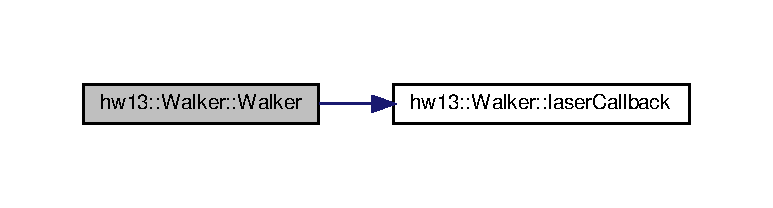
\includegraphics[width=350pt]{classhw13_1_1_walker_a719ac99378e3ddf07b4811058018208d_cgraph}
\end{center}
\end{figure}


\subsection{Member Function Documentation}
\mbox{\Hypertarget{classhw13_1_1_walker_a5675ccfb58c0e78adfad582d840e8f42}\label{classhw13_1_1_walker_a5675ccfb58c0e78adfad582d840e8f42}} 
\index{hw13\+::\+Walker@{hw13\+::\+Walker}!laser\+Callback@{laser\+Callback}}
\index{laser\+Callback@{laser\+Callback}!hw13\+::\+Walker@{hw13\+::\+Walker}}
\subsubsection{\texorpdfstring{laser\+Callback()}{laserCallback()}}
{\footnotesize\ttfamily void hw13\+::\+Walker\+::laser\+Callback (\begin{DoxyParamCaption}\item[{const sensor\+\_\+msgs\+::\+Laser\+Scan\+::\+Const\+Ptr \&}]{data }\end{DoxyParamCaption})}



Laserscan subscriber callback. 


\begin{DoxyParams}{Parameters}
{\em data} & Single scan from a planar laser range finder \\
\hline
\end{DoxyParams}
Here is the caller graph for this function\+:\nopagebreak
\begin{figure}[H]
\begin{center}
\leavevmode
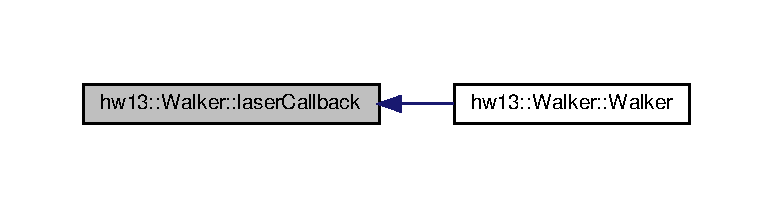
\includegraphics[width=350pt]{classhw13_1_1_walker_a5675ccfb58c0e78adfad582d840e8f42_icgraph}
\end{center}
\end{figure}


The documentation for this class was generated from the following files\+:\begin{DoxyCompactItemize}
\item 
include/\hyperlink{walker_8hpp}{walker.\+hpp}\item 
src/\hyperlink{walker_8cpp}{walker.\+cpp}\end{DoxyCompactItemize}

\chapter{File Documentation}
\hypertarget{walker_8hpp}{}\section{include/walker.hpp File Reference}
\label{walker_8hpp}\index{include/walker.\+hpp@{include/walker.\+hpp}}


Walker class.  


{\ttfamily \#include $<$ros/ros.\+h$>$}\newline
{\ttfamily \#include $<$std\+\_\+msgs/\+String.\+h$>$}\newline
{\ttfamily \#include $<$sensor\+\_\+msgs/\+Laser\+Scan.\+h$>$}\newline
Include dependency graph for walker.\+hpp\+:\nopagebreak
\begin{figure}[H]
\begin{center}
\leavevmode
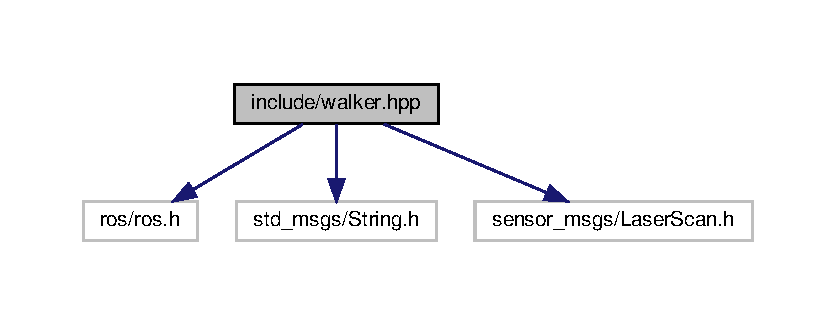
\includegraphics[width=350pt]{walker_8hpp__incl}
\end{center}
\end{figure}
This graph shows which files directly or indirectly include this file\+:\nopagebreak
\begin{figure}[H]
\begin{center}
\leavevmode
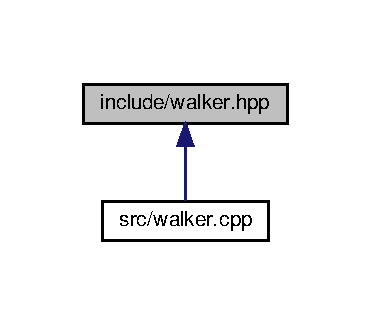
\includegraphics[width=178pt]{walker_8hpp__dep__incl}
\end{center}
\end{figure}
\subsection*{Classes}
\begin{DoxyCompactItemize}
\item 
class \hyperlink{classhw13_1_1_walker}{hw13\+::\+Walker}
\begin{DoxyCompactList}\small\item\em \hyperlink{classhw13_1_1_walker}{Walker} class. \end{DoxyCompactList}\end{DoxyCompactItemize}


\subsection{Detailed Description}
Walker class. 

2021 Markose Jacob

\begin{DoxyAuthor}{Author}
Markose Jacob 
\end{DoxyAuthor}
\begin{DoxyDate}{Date}
11/27/2021
\end{DoxyDate}
\hypertarget{walker_8cpp_LICENSE}{}\subsection{L\+I\+C\+E\+N\+SE}\label{walker_8cpp_LICENSE}
M\+IT License Copyright (c) 2021 Markose Jacob Permission is hereby granted, free of charge, to any person obtaining a copy of this software and associated documentation files (the \char`\"{}\+Software\char`\"{}), to deal in the Software without restriction, including without limitation the rights to use, copy, modify, merge, publish, distribute, sublicense, and/or sell copies of the Software, and to permit persons to whom the Software is furnished to do so, subject to the following conditions\+:

The above copyright notice and this permission notice shall be included in all copies or substantial portions of the Software.

T\+HE S\+O\+F\+T\+W\+A\+RE IS P\+R\+O\+V\+I\+D\+ED \char`\"{}\+A\+S I\+S\char`\"{}, W\+I\+T\+H\+O\+UT W\+A\+R\+R\+A\+N\+TY OF A\+NY K\+I\+ND, E\+X\+P\+R\+E\+SS OR I\+M\+P\+L\+I\+ED, I\+N\+C\+L\+U\+D\+I\+NG B\+UT N\+OT L\+I\+M\+I\+T\+ED TO T\+HE W\+A\+R\+R\+A\+N\+T\+I\+ES OF M\+E\+R\+C\+H\+A\+N\+T\+A\+B\+I\+L\+I\+TY, F\+I\+T\+N\+E\+SS F\+OR A P\+A\+R\+T\+I\+C\+U\+L\+AR P\+U\+R\+P\+O\+SE A\+ND N\+O\+N\+I\+N\+F\+R\+I\+N\+G\+E\+M\+E\+NT. IN NO E\+V\+E\+NT S\+H\+A\+LL T\+HE A\+U\+T\+H\+O\+RS OR C\+O\+P\+Y\+R\+I\+G\+HT H\+O\+L\+D\+E\+RS BE L\+I\+A\+B\+LE F\+OR A\+NY C\+L\+A\+IM, D\+A\+M\+A\+G\+ES OR O\+T\+H\+ER L\+I\+A\+B\+I\+L\+I\+TY, W\+H\+E\+T\+H\+ER IN AN A\+C\+T\+I\+ON OF C\+O\+N\+T\+R\+A\+CT, T\+O\+RT OR O\+T\+H\+E\+R\+W\+I\+SE, A\+R\+I\+S\+I\+NG F\+R\+OM, O\+UT OF OR IN C\+O\+N\+N\+E\+C\+T\+I\+ON W\+I\+TH T\+HE S\+O\+F\+T\+W\+A\+RE OR T\+HE U\+SE OR O\+T\+H\+ER D\+E\+A\+L\+I\+N\+GS IN T\+HE S\+O\+F\+T\+W\+A\+RE.\hypertarget{walker_8cpp_DESCRIPTION}{}\subsection{D\+E\+S\+C\+R\+I\+P\+T\+I\+ON}\label{walker_8cpp_DESCRIPTION}
Header file for Walker Algorithm Class

2021 Markose Jacob

\begin{DoxyAuthor}{Author}
Markose Jacob 
\end{DoxyAuthor}
\begin{DoxyDate}{Date}
11/28/2021
\end{DoxyDate}
\hypertarget{walker_8cpp_LICENSE}{}\subsection{L\+I\+C\+E\+N\+SE}\label{walker_8cpp_LICENSE}
M\+IT License Copyright (c) 2021 Markose Jacob Permission is hereby granted, free of charge, to any person obtaining a copy of this software and associated documentation files (the \char`\"{}\+Software\char`\"{}), to deal in the Software without restriction, including without limitation the rights to use, copy, modify, merge, publish, distribute, sublicense, and/or sell copies of the Software, and to permit persons to whom the Software is furnished to do so, subject to the following conditions\+:

The above copyright notice and this permission notice shall be included in all copies or substantial portions of the Software.

T\+HE S\+O\+F\+T\+W\+A\+RE IS P\+R\+O\+V\+I\+D\+ED \char`\"{}\+A\+S I\+S\char`\"{}, W\+I\+T\+H\+O\+UT W\+A\+R\+R\+A\+N\+TY OF A\+NY K\+I\+ND, E\+X\+P\+R\+E\+SS OR I\+M\+P\+L\+I\+ED, I\+N\+C\+L\+U\+D\+I\+NG B\+UT N\+OT L\+I\+M\+I\+T\+ED TO T\+HE W\+A\+R\+R\+A\+N\+T\+I\+ES OF M\+E\+R\+C\+H\+A\+N\+T\+A\+B\+I\+L\+I\+TY, F\+I\+T\+N\+E\+SS F\+OR A P\+A\+R\+T\+I\+C\+U\+L\+AR P\+U\+R\+P\+O\+SE A\+ND N\+O\+N\+I\+N\+F\+R\+I\+N\+G\+E\+M\+E\+NT. IN NO E\+V\+E\+NT S\+H\+A\+LL T\+HE A\+U\+T\+H\+O\+RS OR C\+O\+P\+Y\+R\+I\+G\+HT H\+O\+L\+D\+E\+RS BE L\+I\+A\+B\+LE F\+OR A\+NY C\+L\+A\+IM, D\+A\+M\+A\+G\+ES OR O\+T\+H\+ER L\+I\+A\+B\+I\+L\+I\+TY, W\+H\+E\+T\+H\+ER IN AN A\+C\+T\+I\+ON OF C\+O\+N\+T\+R\+A\+CT, T\+O\+RT OR O\+T\+H\+E\+R\+W\+I\+SE, A\+R\+I\+S\+I\+NG F\+R\+OM, O\+UT OF OR IN C\+O\+N\+N\+E\+C\+T\+I\+ON W\+I\+TH T\+HE S\+O\+F\+T\+W\+A\+RE OR T\+HE U\+SE OR O\+T\+H\+ER D\+E\+A\+L\+I\+N\+GS IN T\+HE S\+O\+F\+T\+W\+A\+RE.\hypertarget{walker_8cpp_DESCRIPTION}{}\subsection{D\+E\+S\+C\+R\+I\+P\+T\+I\+ON}\label{walker_8cpp_DESCRIPTION}
Header file for Walker Algorithm Class 
\hypertarget{walker_8cpp}{}\section{src/walker.cpp File Reference}
\label{walker_8cpp}\index{src/walker.\+cpp@{src/walker.\+cpp}}


Walker class.  


{\ttfamily \#include $<$ros/ros.\+h$>$}\newline
{\ttfamily \#include $<$std\+\_\+msgs/\+String.\+h$>$}\newline
{\ttfamily \#include $<$sensor\+\_\+msgs/\+Laser\+Scan.\+h$>$}\newline
{\ttfamily \#include \char`\"{}geometry\+\_\+msgs/\+Twist.\+h\char`\"{}}\newline
{\ttfamily \#include \char`\"{}walker.\+hpp\char`\"{}}\newline
Include dependency graph for walker.\+cpp\+:\nopagebreak
\begin{figure}[H]
\begin{center}
\leavevmode
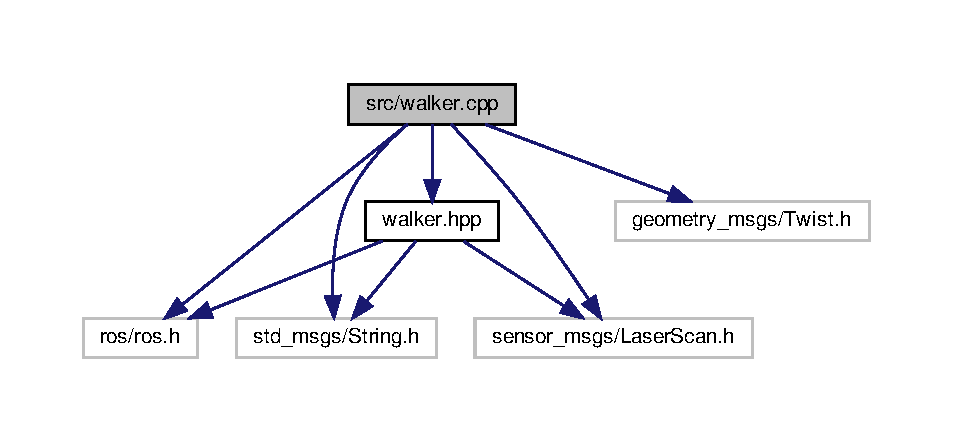
\includegraphics[width=350pt]{walker_8cpp__incl}
\end{center}
\end{figure}


\subsection{Detailed Description}
Walker class. 

2021 Markose Jacob

\begin{DoxyAuthor}{Author}
Markose Jacob 
\end{DoxyAuthor}
\begin{DoxyDate}{Date}
11/28/2021
\end{DoxyDate}
\hypertarget{walker_8cpp_LICENSE}{}\subsection{L\+I\+C\+E\+N\+SE}\label{walker_8cpp_LICENSE}
M\+IT License Copyright (c) 2021 Markose Jacob Permission is hereby granted, free of charge, to any person obtaining a copy of this software and associated documentation files (the \char`\"{}\+Software\char`\"{}), to deal in the Software without restriction, including without limitation the rights to use, copy, modify, merge, publish, distribute, sublicense, and/or sell copies of the Software, and to permit persons to whom the Software is furnished to do so, subject to the following conditions\+:

The above copyright notice and this permission notice shall be included in all copies or substantial portions of the Software.

T\+HE S\+O\+F\+T\+W\+A\+RE IS P\+R\+O\+V\+I\+D\+ED \char`\"{}\+A\+S I\+S\char`\"{}, W\+I\+T\+H\+O\+UT W\+A\+R\+R\+A\+N\+TY OF A\+NY K\+I\+ND, E\+X\+P\+R\+E\+SS OR I\+M\+P\+L\+I\+ED, I\+N\+C\+L\+U\+D\+I\+NG B\+UT N\+OT L\+I\+M\+I\+T\+ED TO T\+HE W\+A\+R\+R\+A\+N\+T\+I\+ES OF M\+E\+R\+C\+H\+A\+N\+T\+A\+B\+I\+L\+I\+TY, F\+I\+T\+N\+E\+SS F\+OR A P\+A\+R\+T\+I\+C\+U\+L\+AR P\+U\+R\+P\+O\+SE A\+ND N\+O\+N\+I\+N\+F\+R\+I\+N\+G\+E\+M\+E\+NT. IN NO E\+V\+E\+NT S\+H\+A\+LL T\+HE A\+U\+T\+H\+O\+RS OR C\+O\+P\+Y\+R\+I\+G\+HT H\+O\+L\+D\+E\+RS BE L\+I\+A\+B\+LE F\+OR A\+NY C\+L\+A\+IM, D\+A\+M\+A\+G\+ES OR O\+T\+H\+ER L\+I\+A\+B\+I\+L\+I\+TY, W\+H\+E\+T\+H\+ER IN AN A\+C\+T\+I\+ON OF C\+O\+N\+T\+R\+A\+CT, T\+O\+RT OR O\+T\+H\+E\+R\+W\+I\+SE, A\+R\+I\+S\+I\+NG F\+R\+OM, O\+UT OF OR IN C\+O\+N\+N\+E\+C\+T\+I\+ON W\+I\+TH T\+HE S\+O\+F\+T\+W\+A\+RE OR T\+HE U\+SE OR O\+T\+H\+ER D\+E\+A\+L\+I\+N\+GS IN T\+HE S\+O\+F\+T\+W\+A\+RE.\hypertarget{walker_8cpp_DESCRIPTION}{}\subsection{D\+E\+S\+C\+R\+I\+P\+T\+I\+ON}\label{walker_8cpp_DESCRIPTION}
Class implementation 
%--- End generated contents ---

% Index
\backmatter
\newpage
\phantomsection
\clearemptydoublepage
\addcontentsline{toc}{chapter}{Index}
\printindex

\end{document}
